\section{Árvore Rubro Negra}
\label{sec:rubro}

Como uma alternativa mais relaxada à Arvore AVL, a Arvore Rubro Negra surgiu do trabalho "A Dichromatic Framework for Balanced Trees"\ de Leonidas J. e Robert Sedgewick, e a escolha das cores rubro e negra foram influenciados pela disponibilidade de canetas dessa cor na época e qualidade de impressão\footnote{\cite{wikipedia_red_black_tree}}.

Para atender a necessidade de se auto balancear, a Rubro-Negra assume algumas regras e características:

\begin{enumerate}
	\item Todo nó é vermelho (rubro) ou preto (negro).
	\item O nó raiz é preto.
	\item Toda folha (\texttt{Nil}) é preta.
	\item Se um nó é vermelho, seus dois filhos são pretos.
	\item Cada caminho da raiz até um nó \texttt{Nil} tem a mesma quantidade de nós pretos.
\end{enumerate}

\begin{figure}[!ht]
	\centering
	\adjustbox{max width=\textwidth}{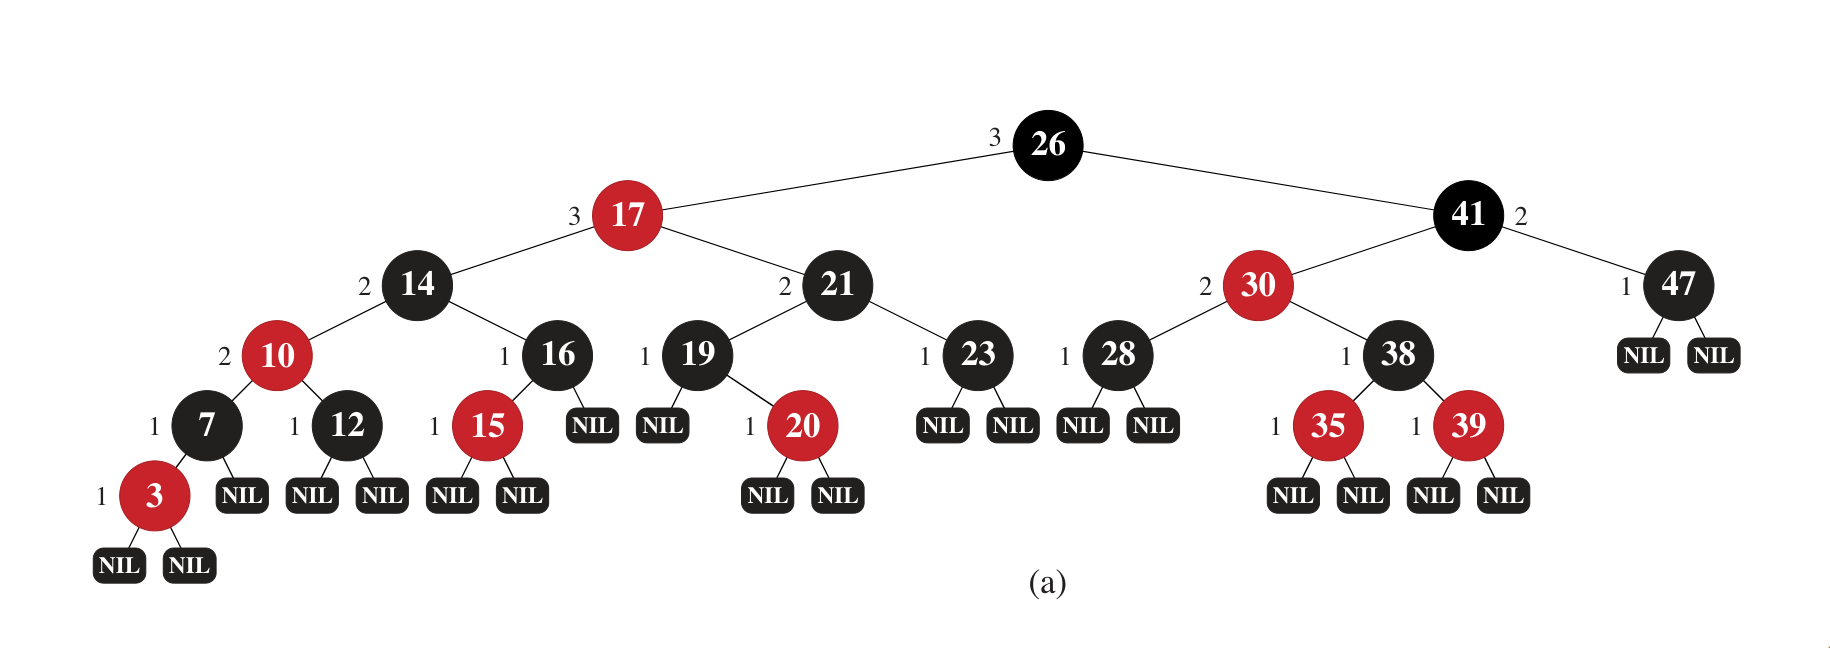
\includegraphics{figures/rubro-negra/example.png}}
	\caption{Imagem retirada de \cite{cormen2022algorithms}}
	\label{fig:rubro_example}
\end{figure}
\FloatBarrier

% TODO: Adicionar nota de rodapé indicando origem da imagem 

Devida sua natureza, uma árvore rubro negra de $n$ elementos tem \textit{profundidade}\footnote{A distância entre um nó qualquer e a raiz} de ao máximo $2\lfloor\log (n + 1)\rfloor$, garantindo que as operações de \textrm{I\textsc{nserção}}, \textrm{B\textsc{usca}}, \textrm{R\textsc{emoção}} tenham complexidade $O(\log n)$ no pior caso.

\subsection{Datatype}

Para sua implementação, usaremos a linguagem de programação Haskell, assumindo a seguinte estrutura.

\begin{lstlisting}[language=haskell, caption={Árvore Rubro-Negra}]
data RBTree a
  = Nil -- black leaf
  | Node Color (RBTree a) a (RBTree a)
  deriving (Show)
\end{lstlisting}

Um elemento do tipo \texttt{RedBlackTree a}, onde '\texttt{a}' é genérico, tem dois construtores: construtor \texttt{Nil}, que implicitamente tem cor preta, ou a função \texttt{Node} aplicada em quatro argumentos, a cor (\texttt{Color}), a árvore esquerda (\texttt{RBTree a}), o valor dentro do nó (\texttt{a}) e a árvore direita (\texttt{RBTree a}),

Neste documento implementaremos a \textrm{I\textsc{nserção}}\footnote{Versão de \cite{okasaki1999functional}} e \textrm{R\textsc{emoção}}\footnote{Versão de \cite{germane2014deletion}}, visto que as implementações da \textrm{B\textsc{usca}} e \textrm{R\textsc{otação}} são análogas a árvore AVL e binária.

\subsection{Implementação da inserção}


Inicialmente, o algoritmo será similar a inserção na Árvore binária convencional, mas uma vez inserido o valor em algum nó, precisamos decidir qual será sua cor e garantir que as regras da Rubro-negra sejam atendidas.

Em relação a cor, insertamos o nó como a cor vermelha, pois minimiza a quantidade de violações. Para garantir que nenhum nó vermelho seja raiz, simplesmente pintamos o último nó de preto. Teremos, então:

\begin{lstlisting}[language=haskell, caption={Função principal}]
insert :: (Ord a) => a -> RBTree a -> RBTree a
insert x tree = blacken (ins tree)
\end{lstlisting}
\FloatBarrier

Naturalmente, os valores que uma Rubro-negra precisa armazenar devem ser ordenáveis (restrição imposta por \texttt{Ord a}), ademais, no primeiro momento, usaremos duas funções auxiliares, a \texttt{blacken} e \texttt{ins}. A \texttt{blacken} será responsável por corrigir a violação anteriormente citada e a \texttt{ins} realizará de fato a inserção, em conjunto com as outras correções.

Começando pela mais simples:

\begin{lstlisting}[language=haskell]
blacken Nil = Nil
blacken (Node _ left r right) = Node Black left r right
\end{lstlisting}
\FloatBarrier

Na \texttt{ins} prosseguimos com uma inserção tradicional em árvore binária, apenas com algumas ressalvas.

\begin{lstlisting}[language=haskell]
ins Nil = Node Red Nil x Nil                 
ins tree@(Node color left r right)           
  | x < r = balance color (ins left) r right 
  | x > r = balance color left r (ins right) 
  | otherwise = tree                         
\end{lstlisting}
\FloatBarrier

Usaremos mais uma função auxiliar chamada \texttt{balance}, que terá a mesma tipagem do construtor \texttt{Node} e será responsável por corrigir as possíveis violações locais causadas pela inserção do novo nó vermelho, as quais:

\begin{itemize}
	\item \textbf{Violação Esquerda-Esquerda:} Dois vermelhos na sub-árvore esquerda. \\
	      Uma vez chegando no caso base e inserindo o valor \texttt{x}, essa violação ocorrerá da seguinte forma:
	      \begin{figure}[!ht]
		      \centering
		      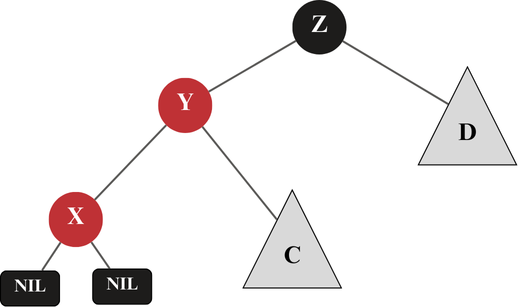
\includegraphics[scale=0.5]{figures/rubro-negra/left-left-insertion.png}
		      \caption{}
	      \end{figure}
	      \FloatBarrier
	      E para resolver localmente essa violação, rotacionamos e alteramos as cores da árvore:
	      \begin{figure}[!ht]
		      \centering
		      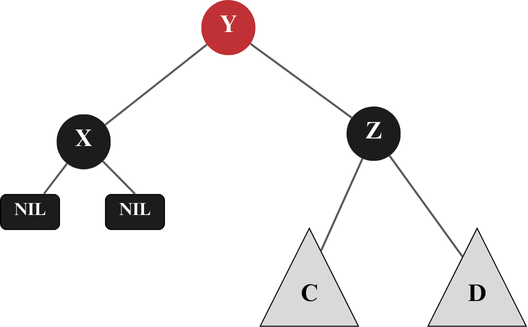
\includegraphics[scale=0.5]{figures/rubro-negra/left-left-base-solution.png}
		      \caption{}
	      \end{figure}
	      \FloatBarrier
	      Entretanto, depois de balancear essa sub-árvore, a raiz vermelha pode ser filho de algum outro nó vermelho na árvore maior. Mas, como a \texttt{balance} é chamada em cada etapa do \texttt{ins}, logo, ela vai continuar corrigindo as violações nas sub-árvores até a topo da árvore. Então generalizamos esse caso:
	      \begin{figure}[!ht]
		      \centering
		      \begin{minipage}{0.4\textwidth}
			      \centering
			      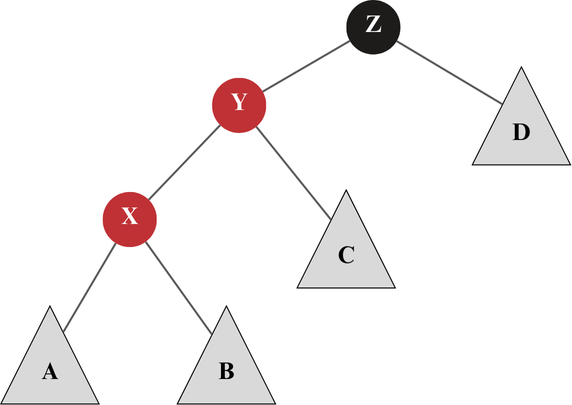
\includegraphics[scale=0.42]{figures/rubro-negra/left-left.png}
			      \caption{}
			      \label{fig:left-left}
		      \end{minipage}%
		      \hspace{1em}
		      \textbf{$\Longrightarrow$}
		      \hspace{1em}
		      \begin{minipage}{0.4\textwidth}
			      \centering
			      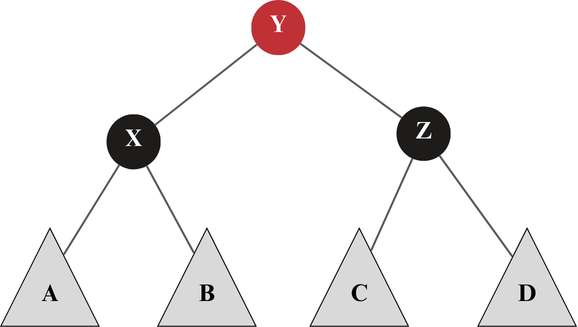
\includegraphics[scale=0.42]{figures/rubro-negra/left-left-solution.png}
			      \caption{}
			      \label{fig:left-left-solution}
		      \end{minipage}
	      \end{figure}
	      \FloatBarrier
	\item \textbf{Violação Esquerda-Direita:} Dois vermelhos, um no filho esquerdo e outro no filho direito do filho esquerdo.
	      \begin{figure}[!ht]
		      \centering
		      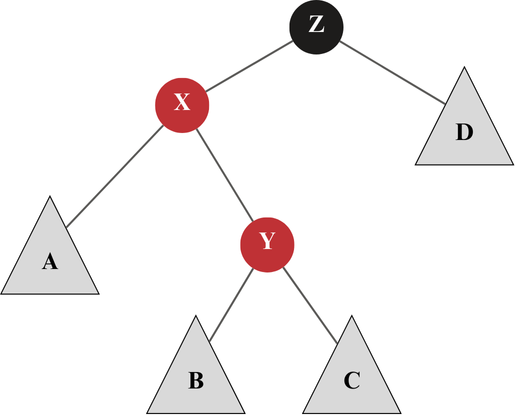
\includegraphics[scale=0.5]{figures/rubro-negra/left-right.png}
		      \caption{}
	      \end{figure}
	      \FloatBarrier
	      Para resolver essa violação, também vamos reconfigurar como foi feito na Figura \ref{fig:left-left-solution}, assim como todas as restantes.
	\item \textbf{Violação Direita-Direita:} Dois vermelhos, na sub-árvore direita.
	      \begin{figure}[!ht]
		      \centering
		      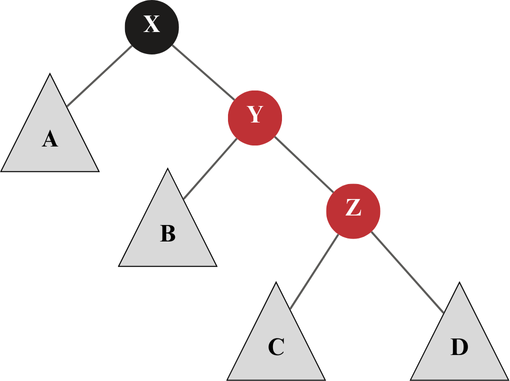
\includegraphics[scale=0.5]{figures/rubro-negra/right-right.png}
		      \caption{}
	      \end{figure}
	      \FloatBarrier
	\item \textbf{Violação Direita-Esquerda} Dois vermelhos, um no filho direito e outro no filho esquerdo do filho direito.
	      \begin{figure}[!ht]
		      \centering
		      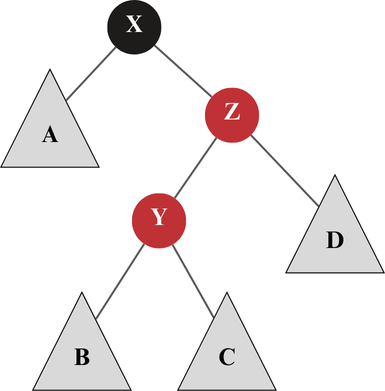
\includegraphics[scale=0.5]{figures/rubro-negra/right-left.png}
		      \caption{}
	      \end{figure}
	      \FloatBarrier
\end{itemize}

\noindent
Uma vez estabelecidos os casos a, implementação desse algoritmo se torna bem mais simples do que versões iterativas, visto que todos os casos produzem o mesmo resultado.

\begin{lstlisting}[language=haskell]
-- Esquerda-Esquerda
balance Black (Node Red (Node Red at x bt) y ct) z dt =
  Node Red (Node Black at x bt) y (Node Black ct z dt)
-- Esquerda-Direita
balance Black (Node Red at x (Node Red bt y ct)) z dt =
  Node Red (Node Black at x bt) y (Node Black ct z dt)
-- Direita-Direita
balance Black at x (Node Red (Node Red bt y ct) z dt) =
  Node Red (Node Black at x bt) y (Node Black ct z dt)
-- Direita-Esquerda
balance Black at x (Node Red bt y (Node Red ct z dt)) =
  Node Red (Node Black at x bt) y (Node Black ct z dt)
-- Padrao
balance color left key right = Node color left key right
\end{lstlisting}
\FloatBarrier

\subsubsection{Teste da implementação:}

Para assertar o funcionamento da Inserção na Árvore Rubro-negra, criaremos uma árvore do zero com o uso desse algoritmo:

\begin{lstlisting}[language=haskell]
fromList :: (Ord a) => RedBlackTree a -> [a] -> RedBlackTree a
fromList = foldr insert
\end{lstlisting}
\FloatBarrier

\noindent
Usando os elementos dessa lista:
$$
	\texttt{[15, 18, 20, 35, 32, 38, 30, 40, 32, 45, 48, 52, 60, 50]}
$$
\begin{figure}[!ht]
	\centering
	\adjustbox{max width=\textwidth}{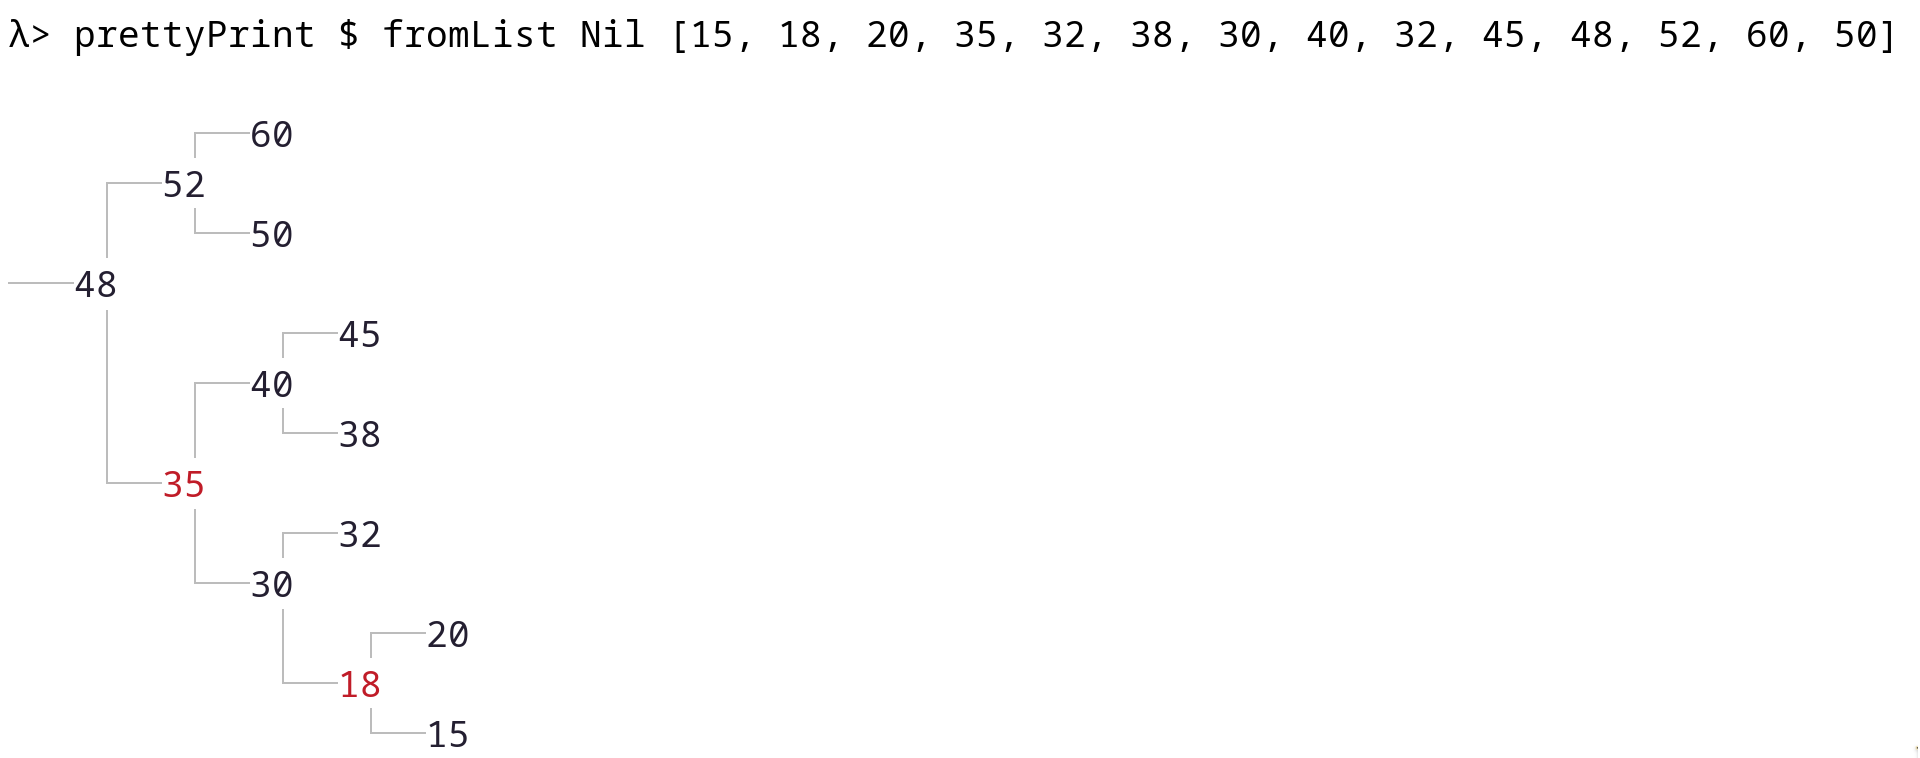
\includegraphics{figures/rubro-negra/insertion-test.png}}
\end{figure}
\FloatBarrier

\subsection{Implementação da remoção}

Assim como na inserção, a remoção na Árvore Rubro-negra tem diversos casos, muitos dos quais são simples de resolver e até idênticos aos da inserção. Entretanto, a remoção de um nó preto sem filho requer uma atenção especial, pois altera a altura da árvore. O truque para lidar com esse caso é adicionar duas cores temporárias '\texttt{BBlack}' e '\texttt{NBlack}', e quebrar-lo em três partes: \textbf{Remoção}, \textbf{Borbulhamento} e \textbf{Balanceamento}.


\begin{enumerate}
	\item Por adicionar a cor '\texttt{BBlack}', o caso se reduz a mudar o nó para uma folha '\texttt{NNil}'. Um nó com cor '\texttt{BBlack}', conta duas vezes a altura de um nó de cor preta, o que permite que a regra seja preservada.
	\item O borbulhamento visa eliminar os '\texttt{BBlack}'s criados pela remoção. As vezes, é possível eliminá-los recolorindo seu pai e irmão. Se não for possível, o '\texttt{BBlack}' é  "borbulhado"\ para seu pai. Para fazer isso, talvez seja necessário recolorir o irmão do nó para '\texttt{NBlack}', caso seja vermelho.
	\item Por fim, o balanceamento elimina os '\texttt{BBlack}'s e '\texttt{NBlack}'s ao mesmo tempo. Generalizamos e usamos a mesma função \texttt{balance} da inserção com dois novos casos.
\end{enumerate}

Representaremos as cores da árvore graficamente como:

\begin{figure}[!ht]
	\centering
	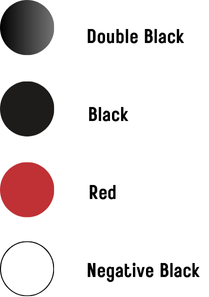
\includegraphics[scale=0.7]{figures/rubro-negra/colors.png}
\end{figure}
\FloatBarrier

E no código como:

\begin{lstlisting}[language=haskell]
data Color
  = Red
  | Black
  | BBlack -- double black
  | NBlack -- negative black
  deriving (Show)
\end{lstlisting}
\FloatBarrier

Para acomodar adição de novas cores, alteramos o datatype da rubro-negra adicionando o construtor \texttt{NNil}, que representa uma folha nula '\texttt{BBlack}'.

\begin{lstlisting}[language=haskell]
data RBTree a
  = Nil -- black leaf
  | NNil -- double black leaf
  | Node Color (RBTree a) a (RBTree a)
  deriving (Show)
\end{lstlisting}
\FloatBarrier

Além disso, para simplificar o algoritmo de remoção, usaremos "aritmética"\ de cores, isto é escurecer e "emvermelhar" uma cor:

\begin{lstlisting}[language=haskell]
blacker Red = Black
blacker Black = BBlack
blacker NBlack = Red
blacker BBlack = error "blacker: too black, received Double Black"

redder NBlack = error "redder: not black enough, received Negative Black"
redder Red = NBlack
redder Black = Red
redder BBlack = Black
\end{lstlisting}
\FloatBarrier



\subsubsection{Primeira parte: Remoção}

Inicialmente começaremos como uma remoção tradicional em um árvore binária, isto é:

\begin{lstlisting}[language=haskell]
remove :: (Ord a, Show a) => a -> RBTree a -> RBTree a
remove x tree = blacken (rem tree)
 where
  rem Nil = Nil
  rem tree@(Node color left r right)
    | x < r = bubble color (rem left) r right
    | x > r = bubble color left r (rem right)
    | otherwise = remove' tree
\end{lstlisting}
\FloatBarrier

Aqui a função \texttt{rem} cumpre papel idêntico ao \texttt{ins} do algoritmo de inserção, entretanto, ao invés de usar diretamente o \texttt{balance}, invocaremos duas partes do nosso algoritmo de remoção, o "Borbulhamento"\ (\texttt{bubble}) e a remoção em si (\texttt{remove'}).

Começando pela remoção, seus casos se agrupam de acordo com quantos filhos o nó alvo tem. Se o nó alvo tem duas sub-árvores, a remoção vai reduzir para o caso em que tem no máximo uma sub-árvore. Para que tal aconteça, encontramos o máximo da sua sub-árvore esquerda, removemos esse nó, e colocamos seu valor no nó a ser removido.

Por exemplo, tome o nó azul como alvo, e o verde como o mais a direita da sub-árvore esquerda do azul.

\begin{figure}[!ht]
	\centering
	\begin{minipage}{0.4\textwidth}
		\centering
		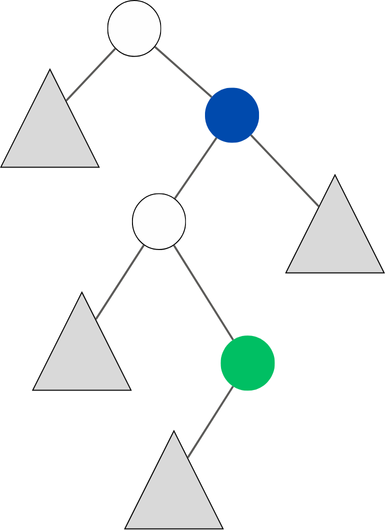
\includegraphics[scale=0.5]{figures/rubro-negra/removal-example.png}
		\caption{}
	\end{minipage}%
	\hspace{1em}
	\textbf{$\Longrightarrow$}
	\hspace{1em}
	\begin{minipage}{0.4\textwidth}
		\centering
		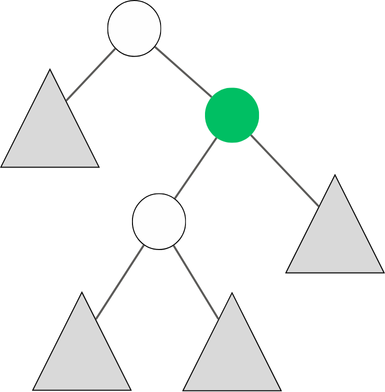
\includegraphics[scale=0.5]{figures/rubro-negra/removal-example-solution.png}
		\caption{}
	\end{minipage}
\end{figure}
\FloatBarrier

Se o nó alvo for uma folha, ou seja, ter filhos \texttt{Nil}, a remoção é imediata.


\begin{figure}[!ht]
	\centering
	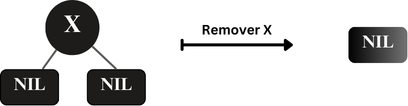
\includegraphics[scale=0.8]{figures/rubro-negra/black-leaf-removal.png}
	\caption{Remoção de folha preta}
	\vspace{3em}
	\centering
	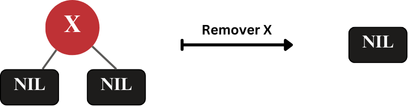
\includegraphics[scale=0.8]{figures/rubro-negra/remove-red-leaf.png}
	\caption{Remoção de folha vermelha}
\end{figure}
\FloatBarrier

Se o nó alvo possuir apenas um filho, existe uma única possibilidade para a esquerda e direita:

\begin{figure}[!ht]
	\centering
	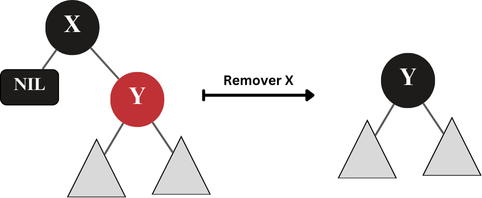
\includegraphics[scale=0.8]{figures/rubro-negra/target-black-one-child.png}
	\caption{Remoção de folha vermelha}
\end{figure}
\FloatBarrier

Em código, definiremos a função \texttt{remove'}, que lidará com esses casos da seguinte forma (em ordem contrária da que eu apresentei):

\begin{lstlisting}[language=Haskell]
remove' Nil = Nil
remove' (Node Red Nil _ Nil) = Nil
remove' (Node Black Nil _ Nil) = NNil
remove' (Node Black Nil _ (Node Red at x bt)) = Node Black at x bt
remove' (Node Black (Node Red at x bt) _ Nil) = Node Black at x bt
remove' (Node color left x right) = 
	bubble color (removeMax left) (max left) right
\end{lstlisting}
\FloatBarrier

A função \texttt{removeMax} remove o elemento mais a direita e a função \texttt{max} vira esse elemento.

\begin{lstlisting}[language=Haskell]
max Nil = error "max: Nil tree, there's no maximum"
max (Node _ _ x Nil) = x
max (Node _ _ x right) = max right

removeMax Nil = error "removeMax: Nil tree, there's no maximum"
removeMax tree@(Node _ _ _ Nil) = remove' tree
removeMax tree@(Node color left x right) = 
	bubble color left x (removeMax right)
\end{lstlisting}
\FloatBarrier



\subsubsection{Segunda parte: Borbulhamento}

O borbulhamento move \texttt{BBlack}'s para os pais, ou elimina-os completamente se possível, no total, existem 6 casos possíveis onde \texttt{BBlack}'s aparecem:

\begin{figure}[!ht]
	\centering
	\adjustbox{max width=\textwidth}{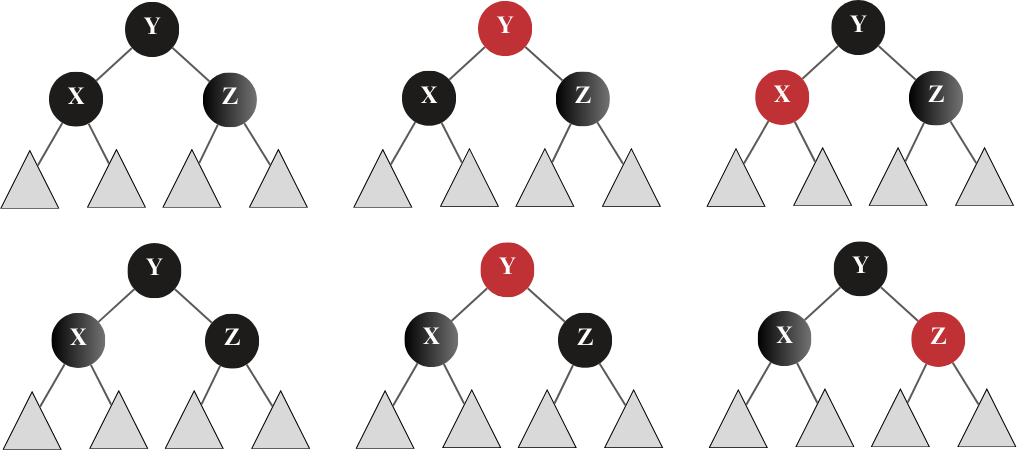
\includegraphics{figures/rubro-negra/bubble-cases.png}}
\end{figure}
\FloatBarrier

Em todos os casos, a ação necessária para mover o \texttt{BBlack} para cima é o mesmo: "Emvermelhar"\ a cor dos filhos e "escurecer"\ a cor dos pais:

\begin{figure}[!ht]
	\centering
	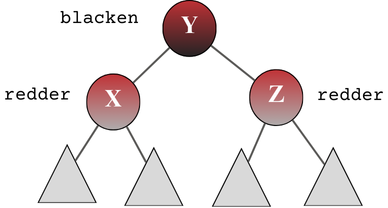
\includegraphics[scale=0.7]{figures/rubro-negra/bubble.png}
\end{figure}
\FloatBarrier

De forma que:

\begin{figure}[!ht]
	\centering
	\adjustbox{max width=\textwidth}{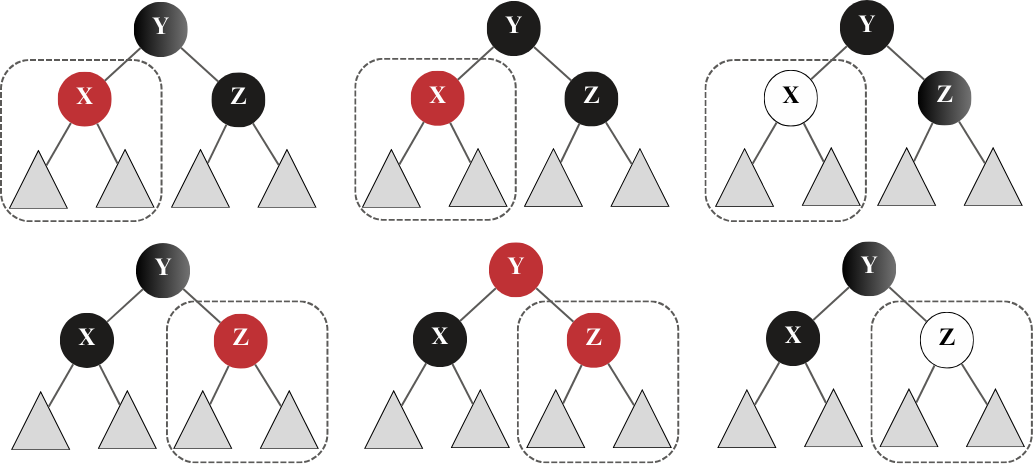
\includegraphics{figures/rubro-negra/bubble-rebalancing-need.png}}
\end{figure}
\FloatBarrier

O pontilhado indica a necessidade de rebalanceamento, a causa é a introdução de uma relacionamento Vermelho-Vermelho ou NBlack/Vermelho entre pai e filho, cujo viola as regras da rubro-negra.

Como toda ação é a mesma, o código da \texttt{bubble} também é relativamente simples:

\begin{lstlisting}[language=Haskell]
bubble :: Color -> RBTree a -> a -> RBTree a -> RBTree a
bubble color left x right
  | isBBlack left || isBBlack right = balance (blacker color) (redder' left) x (redder' right)
  | otherwise = balance color left x right
\end{lstlisting}
\FloatBarrier

A função \texttt{isBBlack} apenas verifica se a árvore tem cor \texttt{BBlack}, e a \texttt{redder'} "opera"\ o vermelho com a árvore, isto é:

\begin{lstlisting}[language=Haskell]
redder' NNil = Nil
redder' (Node color left x right) = Node (redder color) left x right
\end{lstlisting}
\FloatBarrier

\subsubsection{Terceira parte: Balanceamento}

Aqui aproveitamos a \texttt{balance} implementada para a inserção, que consertava essas violações onde a raiz é preta:

\begin{figure}[!ht]
	\centering
	\adjustbox{max width=\textwidth}{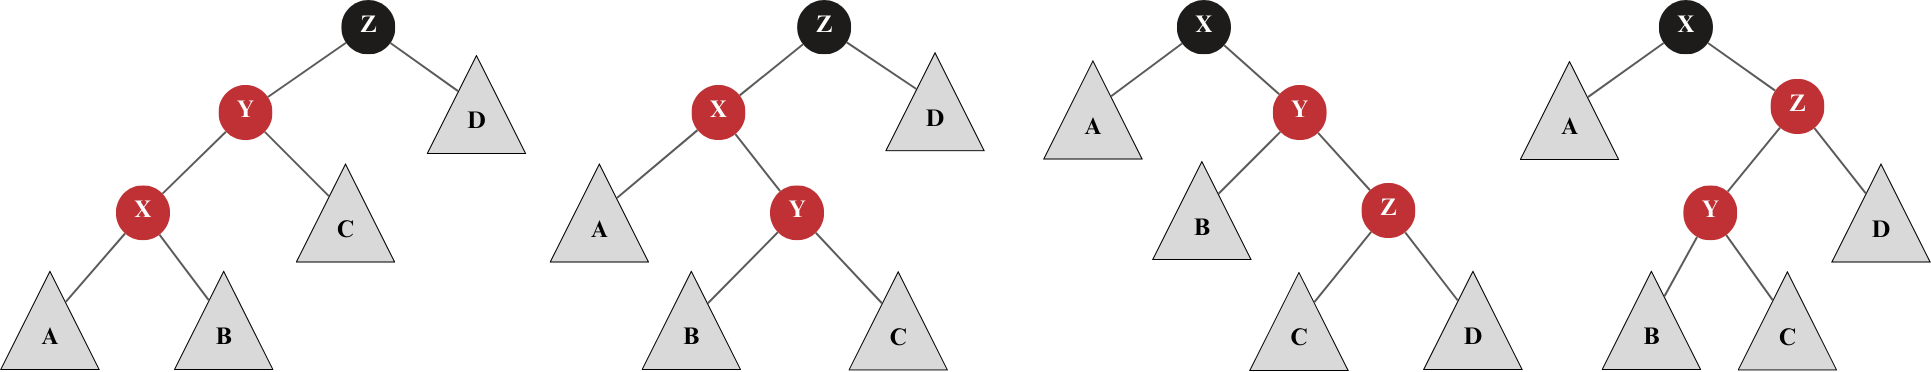
\includegraphics{figures/rubro-negra/balance-insertion.png}}
\end{figure}
\FloatBarrier

Tornando-as nessa árvore:

\begin{figure}[!ht]
	\centering
	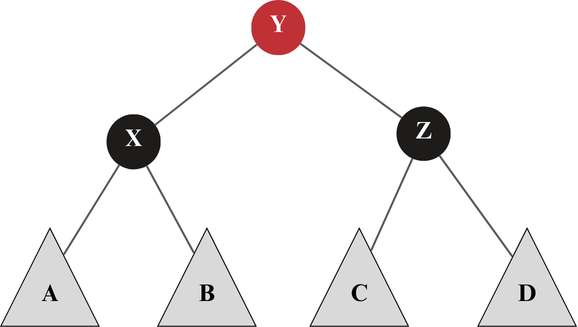
\includegraphics[scale=0.5]{figures/rubro-negra/left-left-solution.png}
\end{figure}
\FloatBarrier

Os novos casos, vão lidar agora com as mesmas violações, mas quando a raiz é \texttt{BBlack}:

\begin{figure}[!ht]
	\centering
	\adjustbox{max width=\textwidth}{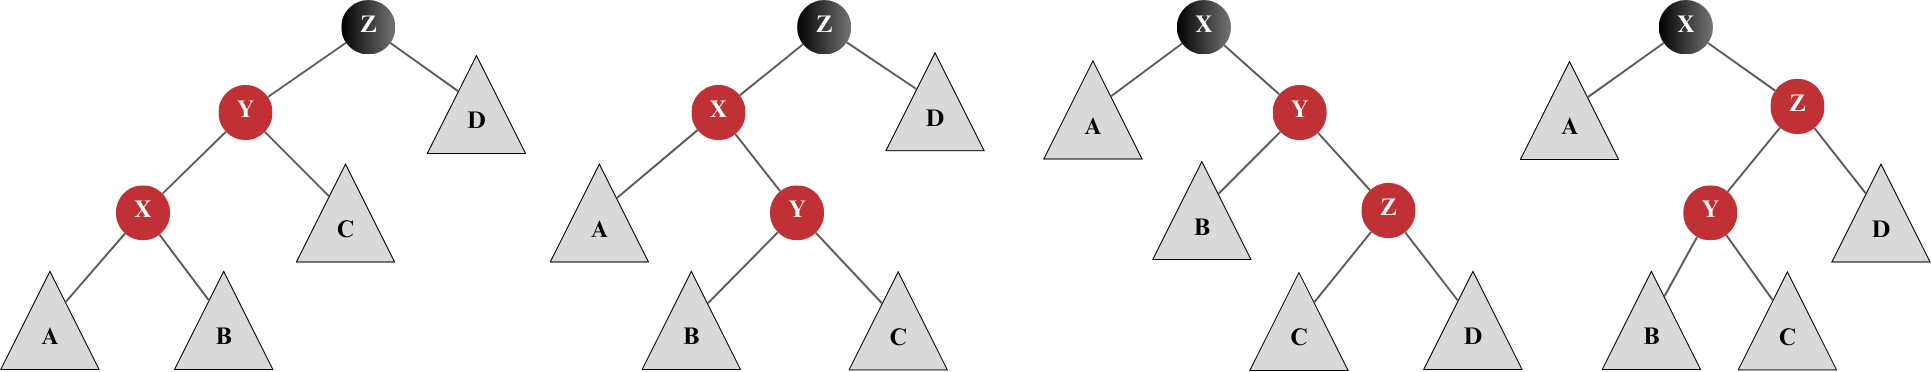
\includegraphics{figures/rubro-negra/balance-removal.png}}
\end{figure}
\FloatBarrier

Transformando todos nessa árvore:

\begin{figure}[!ht]
	\centering
	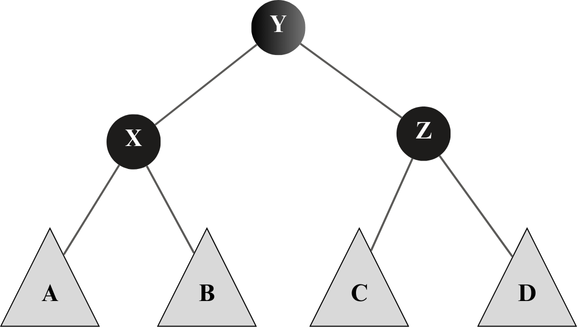
\includegraphics[scale=0.5]{figures/rubro-negra/balance-removal-solution.png}
\end{figure}
\FloatBarrier

Entretanto, se um NBlack aparecer como resultado do Borbulhamento, como em:

\begin{figure}[!ht]
	\centering
	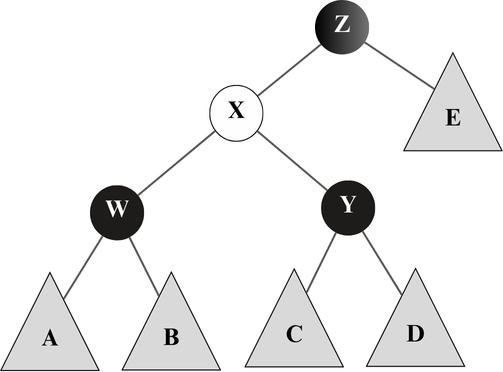
\includegraphics[scale=0.5]{figures/rubro-negra/balance-removal-extra-case.png}
\end{figure}
\FloatBarrier

Uma outra transformação é necessária:

\begin{figure}[!ht]
	\centering
	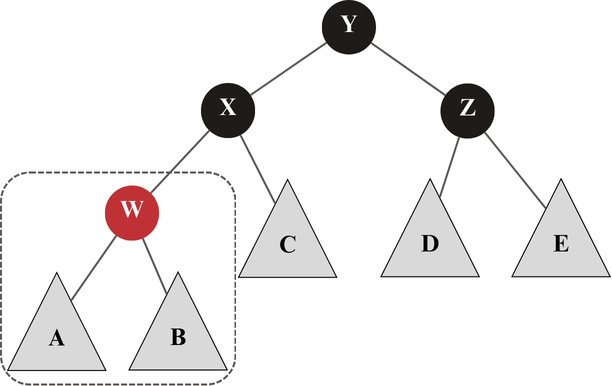
\includegraphics[scale=0.5]{figures/rubro-negra/balance-removal-extra-case-solution.png}
\end{figure}
\FloatBarrier

Novamente, a linha pontilhada indica uma possível violação Vermelho-Vermelho, o que pode precisar de outro rebalanceamento e faz com que a \texttt{balance} precise ser recursiva. Mas, ela não vai se chamar mais de uma vez.
Além disso, existe a versão espelhada dessa última operação. No código, adicionamos os seguintes casos à \texttt{balance}:

\begin{lstlisting}[language=haskell]
-- Violacoes Vermelho-Vermelho com raiz double black
balance BBlack (Node Red (Node Red at x bt) y ct) z dt = 
	Node Black (Node Black at x bt) y (Node Black ct z dt)
balance BBlack (Node Red at x (Node Red bt y ct)) z dt = 
	Node Black (Node Black at x bt) y (Node Black ct z dt)
balance BBlack at x (Node Red (Node Red bt y ct) z dt) = 
	Node Black (Node Black at x bt) y (Node Black ct z dt)
balance BBlack at x (Node Red bt y (Node Red ct z dt)) = 
	Node Black (Node Black at x bt) y (Node Black ct z dt)
-- Casos extra com negative black
balance BBlack at x (Node NBlack (Node Black bt y ct) z dt@(Node Black _ _ _)) =
  Node Black (Node Black at x bt) y (balance Black ct z (redden dt))
balance BBlack (Node NBlack at@(Node Black _ _ _) x (Node Black bt y ct)) z dt =
  Node Black (balance Black (redden at) x bt) y (Node Black ct z dt)
balance color at x bt = Node color at x bt
\end{lstlisting}

Assim, garantimos que todos \texttt{NBlacks}'s sejam removidos e a árvore se mantenha balanceada depois de ter um elemento removido.
